\documentclass[12pt,twoside,a4paper]{uz_ku}
%% опция 'print' для двусторонней печати, 'english' - для статей на английском
%% файл настроен в кодировке UTF8 (все настройки в файле uz_ku.cls - не изменяйте его!)
%% здесь можно добавить НЕОБХОДИМЫЕ авторам пакеты:



%%%%%% Заполняется редакцией %%%%%%%%%%%%%%%%%%%%%%%%%%%%%%%%%%%%%%%%%%%%%%%%%%%%%%%%
\Startpage{1}			% начальная страница (заполняется верстальщиком)			%
\Year{2025}	  			% год														%
\Volume{166}  			% том														%
\Book{1}  				% книга														%
\Type{original} 		% тип: original или review, иначе использовать команду:		%
						% %\SetType{Т\,И\,П~~С\,Т\,А\,Т\,Ь\,И}{A\,R\,T~~T\,Y\,P\,E}	%
\Received{??.??.????} 	% дата поступления в редакцию (без первого нуля)			%
\Accepted{??.??.????}	% дата принятия к публикации  (без первого нуля) 			%
%%%%%% Заполняется редакцией %%%%%%%%%%%%%%%%%%%%%%%%%%%%%%%%%%%%%%%%%%%%%%%%%%%%%%%%

%%%%%%%%%%%%%%% для верстальщика %%%%%%%%%%%%%%%%%%%%%%%%%%%
%% \usepackage{showframe}	% чтобы видеть геометрию 	%%
%% \overfullrule = 3cm   	% чтобы видеть переполнения 	%%								
%%%%%%%%%%%%%%% для верстальщика %%%%%%%%%%%%%%%%%%%%%%%%%%%

\UDK{532.546} 

\InformationInRussian

\TITLE{О процессе выпадения парафина в пласте}
\ShortTITLE{О процессе выпадения парафина в пласте} % первые три-четыре слова и \ldots
\AUTHOR{И.С.~Лазарев \cormail{Lazarevigor.2001@mail.ru}, А.И.~Никифоров}
%% если авторы работают в одном и том же институте - \aff не ставить или \aff{}
%% \cormail - e-mail для корреспонденции, должен быть ровно один и стоять при соответствующем авторе
\CiteAUTHOR[]{Лазарев~И.С., Никифоров~А.И.} %% ИНОЙ порядок инициалов при цитировании! ([опциональный] аргумент - иное название статьи)

%% Пример  оформления  аффилиации (если автор один или у всех авторов общие аффилиации - убрать номер в скобках)
\Affil{Институт механики и машиностроения ФИЦ КазНЦ РАН, г.~Казань, 420111,~Россия}

\Abstract{Предложена математическая модель, описывающая в двумерной постановке процесс отложения парафина при закачке холодной воды в коллектор, насыщенный парафинистой нефтью. Учтены процессы фазовых переходов, связанные с кристаллизацией парафина при снижении температуры, и последующее отложение твердых частиц в пористой среде. Процесс осаждения парафина предполагается равновесным и моделируется на основе теории идеального раствора для двухкомпонентной системы «нефть-парафин». Механизм блокировки пор описан с использованием функции распределения пор по размерам. Полученная система дифференциальных уравнений решалась методом конечных объемов. Для совместного решения уравнений давления и насыщенности был использован метод IMPES (Implicit Pressure Explicit Saturation). Результаты исследования выявили, что кольматация порового пространства парафиновыми отложениями приводит к значительному ухудшению фильтрационно-емкостных свойств пласта. Наблюдается существенное снижение проницаемости и скорости фильтрации флюидов. Это обусловливает уменьшение продуктивности скважин и, как следствие, увеличение продолжительности разработки месторождения.  Также происходит снижение коэффициента извлечения нефти из-за блокировки поровых каналов. В совокупности это сильно снижает эффективность систем поддержания пластового давления, что требует разработки соответствующих методов интенсификации добычи.}

% Ключевые слова на русском:
\KEYWORDS{неизотермическая фильтрация, парафиновые отложения, дисперсные частицы, кольматация, пористость, проницаемость, повреждение пласта, численное моделирование}


% то же самое дублируется на английском языке
\InformationInEnglish

\TITLE{About the process of paraffin deposition in the formation}
\ShortTITLE{About the process of paraffin deposition \ldots} % the first two-three words and \ldots
\AUTHOR{I.S.~Lazarev \cormail{Lazarevigor.2001@mail.ru}, A.I.~Nikiforov}
\CiteAUTHOR[]{Lazarev~I.S., Nikiforov~A.I.}

\Affil{Institute of Mechanics and Mechanical Engineering FIC KazanSC of RAS, Kazan, 420111,~Russia}

\Abstract{A mathematical model is proposed that describes in a two-dimensional formulation the process of paraffin deposition during injection of cold water into a reservoir saturated with paraffin oil. The processes of phase transitions associated with the crystallization of paraffin with a decrease in temperature and the subsequent deposition of solid particles in a porous medium are taken into account. The process of paraffin deposition is assumed to be in equilibrium and is modeled based on the theory of an ideal solution for a two-component oil-paraffin system. The pore blocking mechanism is described using the pore size distribution function. The resulting system of differential equations was solved by the finite volume method. The IMPES (Implicit Pressure Explicit Saturation) method was used to solve the pressure and saturation equations together. The results of the study revealed that the colmatation of the pore space by paraffin deposits leads to a significant deterioration in the filtration and capacitance properties of the formation. There is a significant decrease in the permeability and filtration rate of fluids. This leads to a decrease in well productivity and, as a result, an increase in the duration of field development.  There is also a decrease in the oil recovery coefficient due to the blockage of pore channels. Together, this greatly reduces the efficiency of reservoir pressure maintenance systems, which requires the development of appropriate production intensification methods.}

\KEYWORDS{non-isothermal filtration, paraffin deposits, dispersed particles, colmatation, porosity, permeability, reservoir damage, numerical modeling}


\begin{document}

\section*{Введение}

	В процессе разработки нефтегазовых месторождений заводнением пластовые флюиды могут приобретать температуру, отличную от естественной температуры пласта. Это изменение может быть вызвано различными причинами, зависящими от характера фильтрационного потока, а также от технологии разработки, в процессе которой на продуктивные коллекторы оказывают различные тепловые воздействия. Примером подобного воздействия является нагнетание воды с целью поддержания пластового давления. В случае, когда температура нагнетаемой вода воды ниже температуры пласта, может возникать множество негативных эффектов, ухудшающих фильтрационно-емкостные свойства коллектора. Наиболее яркий пример — отложение парафина, вызывающее снижение пористости, проницаемости, особенно вблизи призабойной зоны пласта, и, следовательно, увеличение скин-фактора [2].
	Нефтяные месторождения высоковязких нефтей, содержащих значительные концентрации парафинов, смол и асфальтенов, осваиваются с меньшей интенсивностью. Это связано с тем, что такие залежи требуют применения специализированных технологий для эффективной добычи, транспортировки и подготовки. Но сложность разработки не уменьшает их экономический потенциал. Глобальные запасы подобных нефтей превышают 810 миллиардов тонн. Россия уступает по этому показателю только Венесуэле и Канаде, обладая геологическими запасами высоковязкой нефти порядка 6-7 миллиардов тонн [1].
	Парафины преимущественно состоят из нормальных алканов с числом атомов углерода $C18$ до $C35$ количество которых в парафине обычно превышает 75\%, а остальная часть в основном состоит из изоалканов, циклоалканов и алкилбензолов [4]. Растворимость парафина в нефти непосредственно связана с ее температурой. При достаточно высокой температуре парафин может полностью раствориться в нефти. В условиях пониженной температуры парафин способен затвердевать, при этом образуется дисперсная система, состоящая из жидкой нефтяной фазы и твёрдых частиц парафина. При промежуточных температурных значениях парафиновый компонент может быть частично растворен в нефти, а частично находиться в нефтяной фазе в виде дисперсных частиц. Образование твердых частиц парафина в нефти сопровождается их осаждением на поверхности пор пласта. Накопление парафиновых отложений приводит к уменьшению проницаемости пористой среды, что значительно затрудняет отбор нефти из пластов.  Таким образом, парафиновые отложения становятся серьезной причиной снижения производительности нефтяных скважин. Анализ керна с применением компьютерной томографии до и после фильтрации парафинсодержащей нефти при пониженной температуре [9] показал, что кольматация порового пространства парафином привела к уменьшению открытой пористости с $C18$ до $C35$  Построение модели прогнозирования осаждения парафина представляет собой комплексную задачу. При моделировании закачки холодной воды в нефтяной пласт необходимо учитывать два основных явления: процесс кристаллизации парафина в нефти и последующий процесс отложения парафина на поверхность пор. Имеется богатый объем информации о теплофизических характеристиках и химическом составе парафиновых соединений [3]. Разработаны различные термодинамические модели, позволяющие предсказать температуру начала кристаллизации (температуру помутнения), и описывать состояние равновесия между твердой и жидкой фазами для углеводородных систем [4-6]. В ряде научных работ для моделирования растворимости/осаждения парафинов применялось уравнение теории реальных растворов для бинарной смеси. В качестве альтернативного подхода во некоторых исследованиях используется теория идеального раствора бинарной смеси [7-8]. Обычно интенсивность отложения частиц парафина представляется комбинацией трех независимый факторов [2, 5-6, 9]. Первый фактор характеризует осаждение частиц на стенках пор под действием силы тяжести и/или адгезии. Второй — выражает вынос парафиновых отложений потоком нефти при превышении определенного порогового значения внутрипоровой скорости. Последний — описывает скорость, с которой парафиновые частицы блокируют поры. Отложение твердых частиц парафина в пористой среде влечет за собой снижение проницаемости. Текущее локальное значение проницаемости определяется степенной зависимостью, схожей с формулой и Козени-Кармана [10].
	В настоящей работе нефть моделируется как двухкомпонентная углеводородная смесь, состоящая из «нефти» и «парафина». Предполагается, что данные компоненты не смешиваются с водой. Для прогнозирования температуры начала кристаллизации парафина применяется модель идеального раствора бинарной смеси [8]. Особое внимание уделяется механизму блокировки пор парафином. Функция распределения пор по размерам используется для определения коэффициентов пористости и проницаемости [3]. Также при помощи нее строятся замыкающие соотношения для уравнений сохранения массы, импульса и энергии [3, 11-12]. 

\section*{Постановка задачи}

Основной текст статьи.
Рисунки могут быть подготовлены в любом графическом редакторе и предоставлены в формате EPS (предпочтительно) или JPG в~хорошем качестве для печати. Сноски оформляются следующим образом\footnote{Пример оформления сноски.}. При использовании номерных ссылок используйте неразрывный пробел: уравнение~\eqref{eq:1} или формула~(1), теорема~\ref{thm:1}, работа~\cite{grom}. 



\subsection{Пример вставки рисунка. }

При вставке рис.~\ref{fig:1} ссылка на него обязательна и располагается в TEX файле в абзаце, предшествующем команде вставки иллюстрации, независимо от того, в каком месте она будет отображена в PDF. Центрирование рисунка происходит автоматически. Подпись к рисунку без точки.

\begin{figure} % не требует центрирования, это уже настроено 
	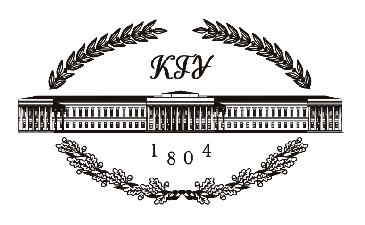
\includegraphics[clip,width=40mm]{fig.eps}
	\bicaption
	{Пример вставки рисунка. Подпись к рисунку ПОД ним,	без точки} % название на русском
	{Example of inserting a figure}						  % перевод на английский
	\label{fig:1}
\end{figure}


\subsection{Пример вставки таблицы. }

При вставке табл.~\ref{tab:2} ссылка на нее обязательна и располагается в TEX файле в абзаце, предшествующем команде вставки таблицы, независимо от того, в каком месте она будет отображена в PDF. Центрирование таблицы происходит автоматически. Название таблицы без точки.

\begin{table} % не требует центрирования, это уже настроено 
	\bicaption
	{Название таблицы размещается СВЕРХУ нее, без точки} % название на русском
	{Table title in English} 							 % перевод на английский
	\label{tab:2}
	\begin{tabular}{|c|cc|}
	\hline
	% после \\ можно ставить \hline или \cline{col1-col2} \cline{col3-col4} ...
	$n$    &  $A$  & $B$ \\ \hline
	1  &  $x$ &  ---  \\
	2  &  $y$ &  $z$ \\ \hline
	\end{tabular}
\end{table}

\section{Название второго раздела}



\begin{Theorem}\label{thm:1}
Формулировка теоремы.
\end{Theorem}

\begin{proof}
Текст доказательства. Пример использования формулы с номером:
\begin{equation}\label{eq:1}
		a(x)=b^3,
\end{equation}
\begin{equation}\label{eq:2}
		c(x)=d^2,
\end{equation}
\begin{equation}\label{eq:3}
		f(x)=\int x^a dx.
\end{equation}
..........
Теорема доказана.
\end{proof}

Возможны ссылки на формулы. Например, здесь мы сослались на формулу~\eqref{eq:1} из предыдущей теоремы~\ref{thm:1}. Пример ссылок на несколько формул~\eqref{eq:1}, \eqref{eq:2} или же \eqref{eq:1}--\eqref{eq:3}.
Пример использования формулы без номера:
	$$F(x)=x-4.$$
Пример задания ссылок на используемую литературу~\cite{kolm, grom} или~\cite{miron, lakes, kolm:2}.

\section*{Заключение}
Заключительный текст статьи. Текст. Текст. Текст. Текст. Текст. Текст. Текст. Текст. Текст. Текст. Текст. Текст. Текст. Текст. Текст. Текст. Текст. Текст. Текст. Текст. Текст. Текст. Текст. Текст. Текст. Текст. Текст. Текст. Текст. Текст. Текст. Текст.  Текст. Текст. Текст. Текст. Текст. Текст. Текст. Текст.



%% указать отсутствие конфликта интересов или раскрыть все потенциальные
%% конфликты интересов, которые могли повлиять на результаты исследования
\ConflictOfInterests{Авторы заявляют об отсутствии конфликта интересов}

\ConflictOfInterests{The authors declare no conflicts of interest}

%%%%%%%%%%%%%%%%%%%%%%%%%%%%%%%%%%%%%%%%%%
%% пример библиографии на русском языке %%
%%%%%%%%%%%%%%%%%%%%%%%%%%%%%%%%%%%%%%%%%%

\begin{thebibliography}{99}
\bibitem{kolm}
\textit{Колмогоров А.Н., Фомин С.В.} Элементы теории функций и функционального анализа. М.: Наука, 1976.  543~с.

\bibitem{grom}
\textit{Громов М.Л.} Красочные категории // УМН. 1970. Т.~70, №~4.  C.~3--76. \URL{https://doi.org/10.4213/rm9657.}

\bibitem{miron}
\textit{Мироненко В.А., Петров Н.С.} Загрязнение подземных вод углеводородами // Геоэкология. 1995.  №~1.  С.~3--27.

\bibitem{lakes}
\textit{Lakes R.} Elastic and viscoelastic behavior of chiral materials // Int. J. Mech. Sci.  2001. V.~43,  No~7.  P.~1579--1589.

\bibitem{kolm:2}
\textit{Kolmogorov A.}  Bemerkungen zu meiner Arbeit «Uber die Summen durch den Zufall bestimmter unabh\"angiger Gr\"ossen» // Math. Ann. 1929. Bd.~102. S.~484--488.
\end{thebibliography}

%%%%%%%%%%%%%%%%%%%%%%%%%%%%%%%%%%%%%%%%%%%%%%%%%%
%% библиография дублируется на английском языке %%
%%    	   (оставить нашему переводчику)		%%
%%%%%%%%%%%%%%%%%%%%%%%%%%%%%%%%%%%%%%%%%%%%%%%%%%

\begin{thebibliography}{99}
\bibitem{kolm}
Kolmogorov~A.N., Fomin~S.V. \textit{Elementy teorii funktsii i funktsional'nogo analiza} [Elements of the Theory of Functions and Functional Analysis]. Moscow, Nauka, 1976. 543~p. (In~Russian)
\bibitem{grom}
Gromov~M.L. Colourful categories. \textit{Russ. Math. Surv.}, 2015, vol.~70, no.~4, pp.~591--655. \URL{https://doi.org/10.1070/RM2015v070n04ABEH004956.}
\bibitem{miron}
Mironenko~V.A., Petrov~N.S. Pollution of groundwater with hydrocarbons. \textit{Geoekologiya}, 1995,  no.~1, pp.~3--27. (In Russian)
\bibitem{lakes}
Lakes R. Elastic and viscoelastic behavior of chiral materials. \textit{Int. J. Mech. Sci.},  2001, vol.~43,  no.~7, pp.~1579--1589. \URL{https://doi.org/10.1016/S0020-7403(00)00100-4.}
\bibitem{kolm:2}
Kolmogoroff A.  Bemerkungen zu meiner Arbeit „\"Uber die Summen zuf\"alliger Gr\"ossen“. \textit{Math. Ann.}, 1930, Bd.~102, S.~484--488. (In German)
\end{thebibliography}


%%% Подробная информация об авторах %%%

\InformationInRussian

\Author{Имя Отчество Фамилия}
\Degree{ученая степень}
	\Position{ученое звание, должность}
	\Org{организация, в которой работает автор}
\Email{xxx@yyy.zzz} 
\ORCID{https://orcid.org/????-????-????-????} 

\Author{Иван Иванович Иванов}
\Degree{доктор физико-математических наук}
	\Position{профессор, заведующий кафедрой <<Перспективные материалы>>}
	\Org{Московский авиационный институт}
	\Position{старший научный сотрудник Института математики и механики им. Н.И. Лобачевского}
	\Org{Казанский $($Приволжский$)$ федеральный университет}
\Email{email@mail.ru} 
\ORCID{https://orcid.org/0000-0001-0002-0003}

\InformationInEnglish

\Author{First name M*. Family name} %% M*. - Middle name initial
\Degree{academic degree}
	\Position{academic title, position}
	\Org{organization to which the author is affiliated}
\Email{xxx@yyy.zzz} 
\ORCID{https://orcid.org/????-????-????-????} 

\Author{Andrey N. Kolmogorov}
\Degree{Doc. Sci. (Physics and Mathematics)}
	\Position{Professor, Faculty of Mechanics and Mathematics}
	\Org{Moscow State University}
\Email{email@mail.ru}
\ORCID{https://orcid.org/0000-0001-0002-0003}

\end{document}

